L'application Stibbons fournit un interprète (ou interpréteur) pour le langage du même nom. Cette interprétation du code se déroule en deux phases~: une de compilation lors du chargement du code, et une d'interprétation de l'arbre abstrait (généré lors de la première phase) lors de l'exécution.

La première phase peut elle-même être découpée en deux parties~:
\begin{itemize}
\item l'analyseur lexical qui «~lit le flot de caractères qui constituent le programme source et les regroupe en séquences de caractères significatives appelées \emph{lexèmes}.~» \cite{compilateurs}~;
\item l'analyseur syntaxique qui, à partir des lexèmes, génère un arbre abstrait qui pourra par la suite être analysé pour être interprété.
\end{itemize}

L'interprétation quant à elle se déroule lors de l'analyse sémantique de l'arbre abstrait, qui exécute les opérations contenues dans les nœuds.

\section{Analyseur lexical}
\label{analyse-lexicale}
L'analyse lexicale vise à produire un flot de jetons qui pourront être analysés par l'analyseur syntaxique. Ces jetons sont des paires composées d'un type de jeton et de la valeur du lexème (par exemple, l'analyse du lexème \verb|12| va générer le jeton \verb|<NUMBER,12>| dans notre cas). Certains lexèmes peuvent générer des jetons qui n'ont pas de valeur (par exemple, le lexème \verb|(| va entraîner la génération du jeton \verb|<(>|).

Nous avons fait le choix d'utiliser l'outil Flex pour notre projet (cf.~\ref{Flex}).

\subsection{Jetons}
Notre analyseur lexical a dans un premier temps généré un nombre limité de jetons. Ainsi, en version 0.1, nous générions seulement 26 jetons différents (dont 5 jetons de littéraux), contre 40 jetons en version 1.0 (dont 7 jetons de littéraux). Ces jetons sont définis dans le code source bison (cf. listing~\ref{parser}) et leur valeur a un type C++ défini par la structure listing~\ref{struct-jeton}. Dans cette structure, l'attribut \verb|tok| correspond au type du jeton (défini par une énumération plus tard) tandis que l'attribut \verb|v| correspond à une valeur. En effet, notre langage ayant un typage dynamique, toutes les valeurs ont un type statique de type \verb|Value|. Ainsi, grâce au polymorphisme, le jeton aura une valeur qui pourra être de type dynamique \verb|Number|, \verb|String|, \verb|Boolean|, etc. tout en gardant un type statique de \verb|Value|. C'est lors de l'analyse sémantique (cf.~\ref{analyse-semantique}) que le type réel du jeton est analysé.

\begin{lstlisting}[label=struct-jeton,caption=Type des valeurs des jetons]
struct {
  stibbons::ValuePtr v;
  stibbons::TreePtr tr;
  int tok;
};
\end{lstlisting}

\subsection{Fonctionnement}
Par défaut, l'analyseur lexical généré par Flex utilise des variables globales et n'est pas réentrant. Dans l'optique d'obtenir un analyseur réentrant, nous avons utilisé l'option \verb|%option c++| et établit le modèle \ref{uml-lexer}.

\begin{figure}[h]
\centering
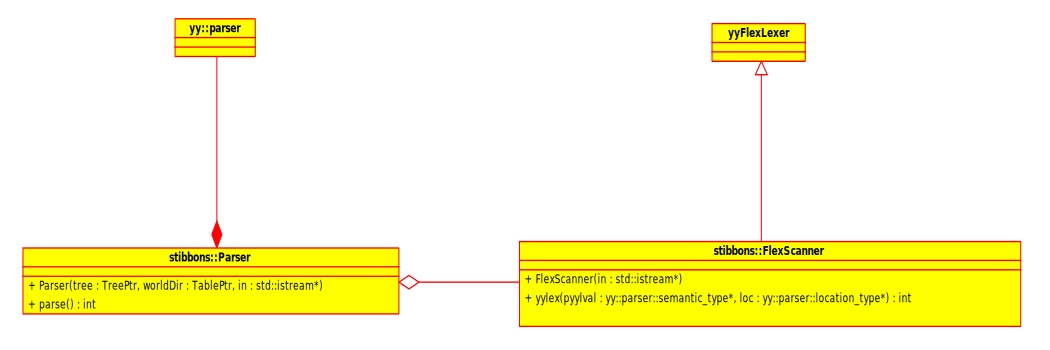
\includegraphics[scale=0.6]{doc/report/img/reentrant-parser}
\caption{\label{uml-lexer} UML des analyseurs lexical et syntaxique}
\end{figure}

Chaque appel à la méthode \verb|yylex()| de \verb|FlexScanner| génère un nouveau token à partir du flux d'entrée passé en paramètre lors de la construction de l'objet \verb|FlexScanner|. Cette méthode analyse le flux à partir des règles définies dans le fichier \verb|lexer.l+| (cf. listing~\ref{lexer}). Ainsi, les instructions définies pour chaque règle sont effectuées quand une chaîne de caractères correspondante à la règle est détectée. Ainsi, dans l'extrait \ref{lex-extrait}, lorsque l'analyseur détecte le caractère \verb|#| suivi d'une séquence de 3 ou 6 nombres hexadécimaux, l'appel au constructeur de \verb|Color(string)| est effectué. Ce dernier crée une couleur à partir d'une chaîne de caractère respectant les codes de couleur html.

\begin{lstlisting}[label=lex-extrait,caption=Exemple de séquence d'instruction lors de la détection d'une couleur]
#([a-f0-9]{6}|[a-f0-9]{3}) {
                           pyylval->v=make_shared<stibbons::Color>(yytext);
                           return yy::parser::token::COLOR;
                           }
\end{lstlisting}

De plus, l'instruction \verb|loc->step()| est effectuée au début de chaque appel à \verb|yylex()|, et permet de faire avancer la position actuelle de la longueur du lexème détecté, et l'instruction \verb|loc->lines()| est effectuée lors de la détection d'un retour à la ligne afin de faire avancer de \verb|n| lignes la position actuelle (avec \verb|n| le nombre de retour à la ligne détecté).
Les différentes règles flex peuvent être consultées au listing \ref{lexer}, ou de façon plus lisible dans l'annexe \ref{flex-rail}.


\section{Analyseur syntaxique}
\label{analyse-syntaxique}
L'analyse syntaxique permet de vérifier que la structure d'un programme est bien en accord avec les règles de grammaire du langage. Par exemple, la grammaire de notre langage comporte une règle, qui indique qu'un appel de fonction sans paramètre, est constituée du jeton \verb|<ID>| suivi des jetons \verb|<(>| et \verb|<)>|. Le but de notre analyse ici est double~: vérifier que le programme est bien un programme de notre langage valide, mais également générer un arbre abstrait qui pourra facilement être analysé par notre analyseur sémantique.

Nous avons fait le choix d'utiliser GNU Bison (cf.~\ref{Bison}) dans notre projet.

\subsection{Arbre abstrait}
Un arbre abstrait est une structure d'arbre dont chaque noeud feuille représente les opérandes des opérations contenues sur les autres noeuds. Cet arbre peut être considéré comme une forme de code intermédiaire, et peut être interprété très facilement en parcourant, pour chaque noeud, les sous-arbres et en appliquant l'opération du noeud courant.

\begin{figure}[h!]
\centering
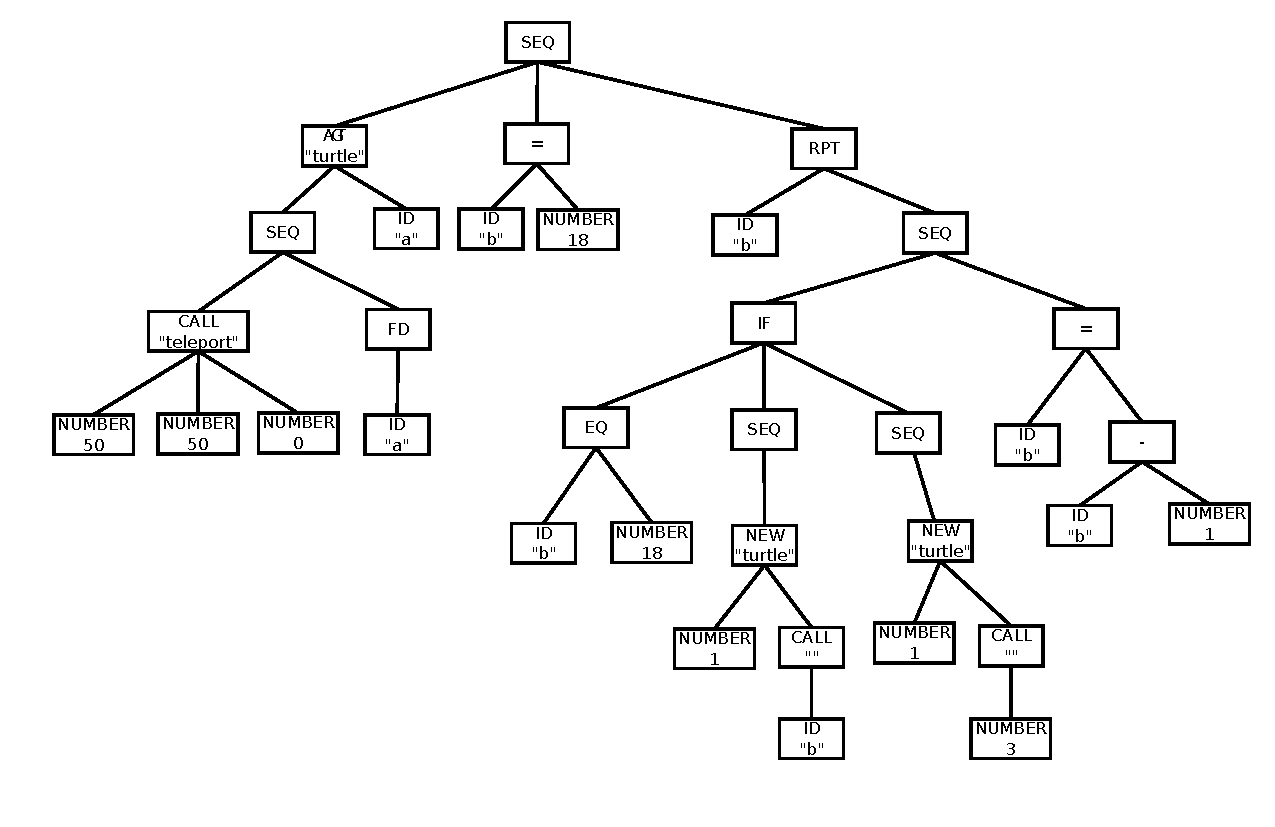
\includegraphics[scale=0.8]{doc/report/img/arbre-abstrait}
\caption{\label{arbre-abstrait} Arbre abstrait généré lors de l'analyse du code \ref{arbre-code}}
\end{figure}
\begin{lstlisting}[language=Stibbons,label=arbre-code,caption=Exemple de code Stibbons]
  agent turtle (a) {
    teleport(50,50,0)
    fd a
  }

  b = 18
  repeat b {
    if(b == 18) {
      new turtle(b)
    }
    else {
      new turtle(3)
    }
    b = b - 1
  }
\end{lstlisting}

L'avantage de générer un tel arbre est qu'il est bien plus rapide d'effectuer un parcours d'arbre à chaque interprétation plutôt que de refaire une analyse syntaxique à chaque fois.

\subsection{Fonctionnement}
L'écriture du fichier Bison est assez semblable au fichier Flex. En effet, on peut associer à chaque règle une liste d'instructions qui vont être exécutées lors de la détection de la règle. Ces instructions peuvent en outre être des affectations de valeur sémantique à une expression. Ainsi, dans l'extrait de code \ref{bison-extrait}, la valeur sémantique d'une sélection est un arbre dont les enfants sont dans l'ordre~: l'expression de test, la séquence d'instructions à exécuter si la condition est vrai et, optionnellement, la séquence d'instructions à exécuter si la condition est fausse.

\begin{lstlisting}[label=bison-extrait,caption=Cas du IF en Bison]
selection : IF expr statement 
{
  stibbons::TreePtr t1 = make_shared<stibbons::Tree>(yy::parser::token::IF,nullptr);
  t1->addChild($2);
  t1->addChild($3);
  t1->setPosition({@1.begin.line,@1.begin.column});
  $$ = t1;
}
| IF expr statement ELSE statement
{
  stibbons::TreePtr t1 = make_shared<stibbons::Tree>(yy::parser::token::IF,nullptr);
  t1->addChild($2);
  t1->addChild($3);
  t1->addChild($5);
  t1->setPosition({@1.begin.line,@1.begin.column});
  $$ = t1;
};
\end{lstlisting}

Bison génère à partir de ces règles un analyseur syntaxique LALR (\emph{look-ahead left-to-right rightmost derivation}). L'analyse du code et la génération de l'arbre sont lancées par un appel à la méthode \verb|stibbons::Parser::parse()| qui va elle-même faire appel à la méthode \verb|yy::parser::parse()|. L'ensemble du code va être analysé, cette méthode se chargeant de faire appel à la méthode \verb|stibbons::FlexScanner::yylex()|, générant et analysant les jetons en une seule passe.


\section{Analyseur sémantique}
\label{Analyseur sémantique}
L'analyse sémantique du Stibbons est effectué dans les classes Interpreter. Plus exactement dans 3 classes. Voir l'UML~\ref{interpreterUML} correspondant page~\pageref{interpreterUML}.

\begin{figure}[h]
\caption{\label{interpreterUML} UML de l'analyseur sémantique}
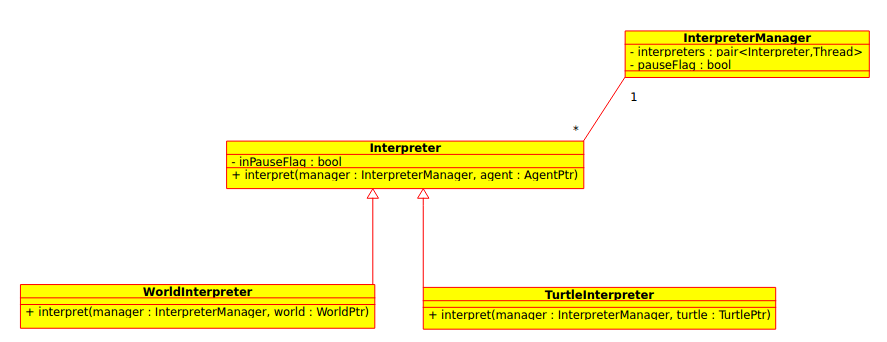
\includegraphics[scale=0.5]{doc/report/uml/interpreterUML.png}
\end{figure}

On a donc les classes \verb|TurtleInterpreter| et \verb|WorldInterpreter| qui héritent de la classe \verb|Interpreter|. Cette dernière analyse et provoque, dans le modèle, les actions liées au code stibbons écrit. Elle permet de gérer tout type d'interaction, du moment que ces actions ne sont pas liées à un monde ou une tortue. La classe \verb|TurtleInterpreter|, gère justement ce dernier type d'actions : celles liées à une tortue. Contrairement à \verb|WorldInterpreter| qui gère les actions du monde.

L'utilité de la classe \verb|InterpreterManager| est expliqué de manière détaillée dans la section \ref{remaniementInterpreter} (page~\pageref{remaniementInterpreter}).

Ainsi, pour avoir un exemple concret, si on demande à une tortue d'avancer en stibbons (ex : \verb|fd 10|), alors c'est le \verb|TurtleInterpreter| qui gèrera cette action.
A contrario, si on effectue une définition de fonction (ex : \verb|a = 10|) alors l'\verb|Interpreter| affectera la valeur \verb|10| à la propriété \verb|a| de l'agent courant.
Pour ce qui est du WorldInterpreter, il n'y a pas encore d'exemple possible, tout simplement car pour l'instant il n'y a pas d'actions spéciales pour le monde.

\subsection{Fonctionnalités}

\subsubsection{Sprint 1 \& 2}
Les deux premiers sprints ont été assez conséquent au niveau du nombre de fonctionnalités ajoutées.
En effet lors du sprint 1 on pouvait déjà effectuer les opérations de bases sur une tortue, telles que avancer, tourner, écrire, etc. De plus les opérations de calculs ainsi que la gestions de nombre ont été fait. En effet, il était nécessaire de gérer les nombres de manière à pouvoir indiquer à la tortue de quelle distance elle devait avancer.

Lors du deuxième sprint sont apparu les conditionnelles, ainsi que les boucles, les comparaisons binaires, les booléens et autres type (color, string, etc.), la création de nouveaux agents dans le code et les fonctions sans paramètres. Ce sprint fut alors une version déjà bien avancé de notre programme final.


\subsubsection{Sprint 3 à 5}
Les sprints suivants ont été plus léger. Non pas parce qu'il y avait moins de travail, car la gestion de l'interpréteur fut remanier à ce moment là, mais car il y avait moins de fonctionnalités à ajouter. En effet à partir du sprint 3, les fonctionnalités suivantes ont été rajoutés~:
\begin{itemize}
\item accès à la parenté et aux zones (en lecture seulement)~;
\item ajout des tables et de boucles dédiés (\verb|foreach|)~;
\item gestion de la vitesse et de la pause~;
\item ajout des communications avec le \verb|send| et le \verb|recv|.
\end{itemize}


\subsection{Remaniement de l'analyseur sémantique}
\label{remaniementInterpreter}

L'analyseur sémantique a d'abord été une seule classe~: la classe \verb|Interpreter|.
Cette dernière implémentait tout types d'actions a effectué pour n'importe quel type d'agent.
Cependant, lors de l'arrivé de la fonctionnalité d'ajout d'un nouvel agent (\verb|new agent|), nous nous sommes aperçu qu'il serait mieux d'avoir un interpréteur par type d'agent, ou plus précisement un interpréteur pour le monde, un pour les tortues et un pour les actions communes aux deux types.
Nous avons alors crée les deux classes~: \verb|WorldInterpreter| et \verb|TurtleInterpreter|.

De manière parallèle, la création du monde s'effectuait dans l'\verb|Interpreter|, puis dans le \verb|WorldInterpreter|, il fut alors nécessaire de crée une classe qui gérerait à la fois la création du monde et tout ce qui concernait l'application (la pause, le temps, les interpreteurs eux-mêmes). Nous avons alors décidé de crée la classe \verb|InterpreterManager|.
Cette classe connait ainsi tout les interpréteurs, permet de les prévenir d'une éventuelle pause du programme, de stocker les threads correspondants à chaque interpréteur, de crée un monde avec les pré-directives choisies~; c'est une sorte de gestionnaire d'interpréteurs.

